\documentclass{article}
\usepackage{graphicx}
\usepackage{amsmath}
\usepackage{float}
\title{Applied Statistical Analysis - ProblemSet 4}
\date{2024-11-17}
\author{Eoghan O'Sullivan}

	\begin{document}
	\maketitle
	\pagenumbering{gobble}
	%\newpage
	%\pagenumbering{arabic}
	
	\section{Question 1}
	I read in the data from its library and made it a data frame called "df" using R statistical software. From there, I wrangled the data and below are the results I produced using the object df. This was done to study whether individuals with higher levels of income have more prestigious jobs than blue and white collar workers, in the context of Canadian occupations.
	\subsection{Part a}
	\paragraph{Create a new variable professional by recoding the variable type so that professionals are coded as 1, and the blue and white collar workers are coded as 0. (Hint: ifelse).}
	The method I used was ifelse applied to the type variable with contained missing data, prof, bc and wc. I ignored the missing data from being coded as 1/0. The bc and wc were 0 and prof accordingly, 1. Figure 1 shows these data.
	\begin{figure}[H]
		\centering
		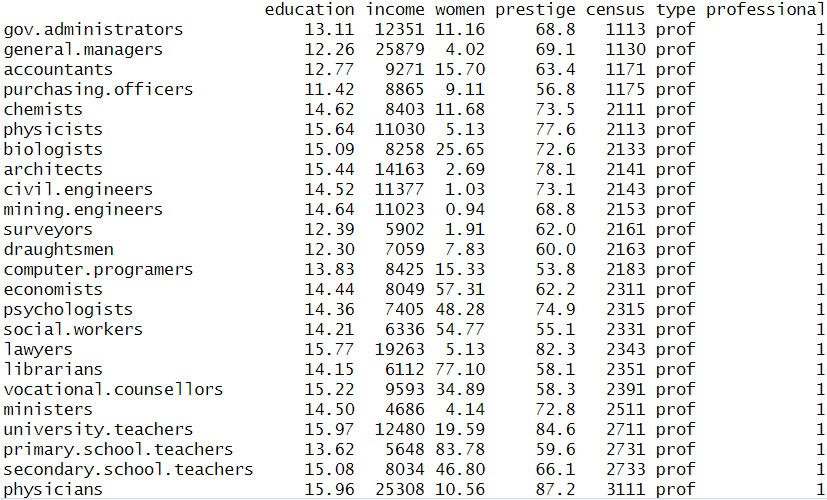
\includegraphics[width=0.9\linewidth]{Data frame printed.jpg}
		\caption{Data}
		\label{fig:Coded new variable called professional}
	\end{figure}
	\subsection{Part b}
	\paragraph{Run a linear model with prestige as an outcome and income, professional, and the interaction of the two as predictors (Note: this is a continuous x dummy interaction.)}
	The results of this are shown in the Figure 2. 
	\begin{figure}[h!]
		\centering
		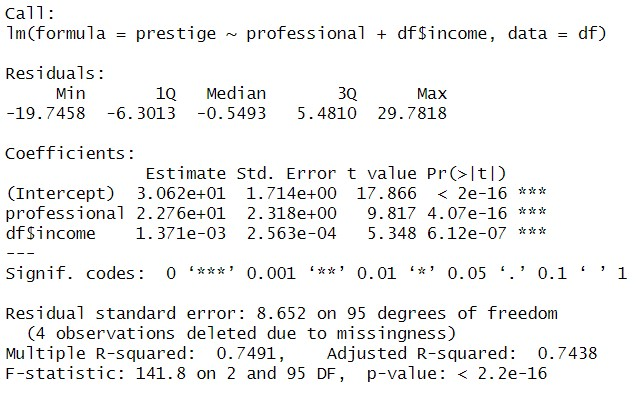
\includegraphics[width=0.9\linewidth]{Regression statistical model.jpg}
		\caption{Regression statistics.}
		\label{fig:Regression statistics.}
	\end{figure}
	\subsection{Part c}
	\paragraph{Write the prediction equation based on the result.}
	I wrote the prediction equation as follows, having calculated the intercept as 
	\begin{equation}
		\beta o
	\end{equation} 
	\paragraph{}and the slopes, as 
	\begin{equation}
		\beta_1 , \beta_2
	\end{equation}The equation is:
	\begin{equation}
		\text{prestige} = \beta_0 + \beta_1 \cdot \text{professional} + \beta_2 \cdot \text{income}
	\end{equation}
	\subsection{Part d}
	\paragraph{Interpret the coefficient for income.}
	I have calculated the coefficient which represents the change in the prestige variable for a one-one increase in income, holding the other variables constant. Given that it is positive, an increase in income is associated with an increase in prestige. The number however is very small, 0.001371 units, for a one-unit increase. There is statistical significance evident as seen by a tiny p-value shown in Figure 2. 
	\subsection{Part e}
	\paragraph{Interpret the coefficient for professional.}
	What is indicated is that being professional is associated with an increase of 22.76 units in prestige, holding other variables constant. The variance has been calculated as being reasonably precise. The p-value is extremely small - well below the common significance threshold of 0.05, so statistical significance is there. There is strong evidence that being professional has an effect on prestige.
	\subsection{Part f}
	\paragraph{What is the effect of a dollar amount increase of 1,000 on prestige in income score for professional occupation? In other words, we are interested in the marginal effect of income when the variable professional takes the value of 1. Calculate the change in $\hat{y}$ associated with a 1,000 dollar increase in income based on your answer for part c.} To do so for this task, I multiplied the income coefficient, 1.371e-03 by 1000, the change in income and printed the result from R. It is 1.371.
	\subsection{Part g}
	\paragraph{What is the effect of changing one's occupation from non-professional to professional when her income is \$6,000? We are interested in the marginal effect of professional jobs when the variable income takes the value of 6,000. Calculate the change in $\hat{y}$ based on your answer for part c.}It is simply the coefficient from before. Answer: 136560. 
	\section{Question 2}
	Without data to analyze, I used the results of a regression with two variables and a constant as provided. The question asked whether the existence of yard signs affect voter share for two candidates and what follows is the conclusions, based on calculations in R.  
	\subsection{Part a}
	\paragraph{Use the results from a linear regression to determine whether having these yard signs in a precint affects vote share (e.g., conduct a hypothesis test with a = .05).}
	The hypothesis test was set up as follows. The null hypothesis is such that coefficient of yard signs is zero (i.e., yard signs do not affect vote share). The alternative hypothesis is that the coefficient of yard signs is not zero (i.e., yard signs affect vote share). Using the provided results of the linear regression, I extracted the coefficient and standard error and completed a t-test. The formula and equation are provided below. 
	\begin{equation}
		t = \frac{Coefficient}{Standard Error} = \frac{0.042}{0.016} = 2.625
	\end{equation}
	So, not zero. I then found the p-value by taking the negative of the absolute value function, abs(). Enclosed is the code. Given that the p-value is below the threshold, I am confident that having yard signs in a precinct affects vote share.  
	\subsection{Part b}
	\paragraph{Use the results to determine whether being next to precincts with these yard signs affects vote share (e.g., conduct a hypothesis test with a = .05).}
	Null Hypothesis is that the coefficient of precinct adjacent to lawn signs is zero (i.e., being adjacent to precincts with yard signs does not affect vote share).
	Alternative Hypothesis is that the coefficient of precinct adjacent to lawn signs is not zero (i.e., being adjacent to precincts with yard signs affects vote share). I extracted the coefficient and standard error and plugged it into R. From it, I calculated the t-value, determined the p-value from it and the degrees of freedom. Comparing the p-value to the significance level (here 0.05) led to rejecting the null hypothesis. So, the coefficient of precinct adjacent to lawn signs is not zero and thus, being adjacent to precincts with yard signs affects vote share.
	\subsection{Part c}
	\paragraph{Interpret the coefficient for the constant term substantively.}
	The intercept value of 0.302 represents the expected value of vote share when both independent variables (precinct assigned lawn signs and precinct adjacent to lawn signs) are zero. So, when there are no yard signs assigned or adjacent (i.e., the variables are zero), the predicted vote share is 30.2 percent.
	This 30.2 percent vote share serves as a baseline measurement. It suggests that, in precincts without the influence of yard signs (neither assigned nor adjacent), the average vote share is expected to be 30.2 percent.
	The standard error of 0.011 indicates the precision of the intercept estimate. A small standard error implies the intercept is estimated with high precision.
	This means there's relatively little variation in the baseline vote share estimate when the influence of yard signs is not present.
	\subsection{Part d}
	\paragraph{Evaluate the model fit for this regression. What does this tell us about the importance of yard signs versus other factors that are not modeled?} The t-value and p-value have been derived from the coefficients and based on the results: yard signs significantly impact vote share both directly and indirectly (adjacent precincts). This highlights their importance relative to other factors, though further data could provide a more comprehensive understanding.
\end{document}